\section{Wait and Notify System}
\subsection{Purpose}
In the current state of DocetOS there is one universal waiting list which, when the notify SVC interrupt is triggered, will wake all currently waiting task regardless of whether the item blocking the task is free. Most tasks from the waiting list will then immediately re-enter the waiting list after discovering they still need to wait for a resource to become available. By separating the main waiting list into a separate waiting list for each blocking item (mutex, semaphore, etc.) we can greatly improve the efficiency of task notification.

\subsection{Specification and Design Considerations}
Tasks must be moved from the scheduler to a specified waiting list, and the blocking item containing the waiting list needs to be capable of notifying the task at the front of the waiting list, returning the task to the scheduler, pre-empting the currently running task if the notified task has a higher priority. To retain mutual exclusivity of the scheduler, task movement to/from waiting lists must be done using SVC interrupts.

\subsection{Implemented Design and Functionality}
\subsubsection{Waiting List Data Structure}

%\setlength\intextsep{0pt}
\begin{wrapfigure}{r}{0.4\textwidth}
	\centering
	\vspace{-\baselineskip}
	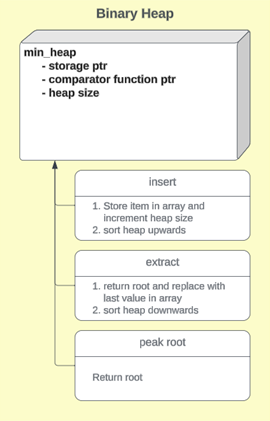
\includegraphics[width=0.4\textwidth]{heap}
\end{wrapfigure}

To implement the improved waiting system, a binary heap module is provided that contains the functionality required to initialise and manage an ordered heap which can be individualised to specific use cases by providing the heap with a comparison function. Using a heap, gives the ability to notify the single item that needs to be notified next instead of the entire waiting list, improving notification efficiency. \hfill\newline
For a blocking item to integrate the waiting list feature, it must declare a waiting list and provide a comparator function, choosing to order the waiting list by a range of task properties including time in the queue, priority, and wake-time. \hfill\newline
The binary heap data structure is used in various applications throughout the operating system, including within the scheduler. So, by consolidating binary heap logic into a generic heap module, the usage of heaps is simplified system wide.

\subsubsection{Task Waiting and Notification}
To give blocking items the ability to wait/notify tasks, SVC interrupt handlers are added to the Fixed-Priority Scheduler that facilitate the movement of tasks between waiting lists and the scheduler. By utilising an SVC interrupt, we maintain the mutual exclusivity of the scheduler while providing a function that can be easily called anywhere within the OS.